% Source: graduate-coursework/Research/How_to_write/00_Contrastive_Synthesis.tex
% Description: \textbf{McEnerney's Reader-Value Model (2014).

\documentclass[border=4pt]{standalone}
\usepackage{newtxtext,newtxmath}
\usepackage{tikz}
\usetikzlibrary{arrows.meta,positioning,shapes.geometric,calc,decorations.pathreplacing}

\definecolor{garnet}{HTML}{73000A}
\definecolor{atlantic}{HTML}{466A9F}
\definecolor{congaree}{HTML}{1F414D}
\definecolor{horseshoe}{HTML}{65780B}
\definecolor{rose}{HTML}{CC2E40}
\definecolor{honeycomb}{HTML}{A49137}
\definecolor{warmgrey}{HTML}{676156}
\definecolor{black90}{HTML}{363636}
\definecolor{black70}{HTML}{5C5C5C}
\definecolor{black50}{HTML}{A2A2A2}
\definecolor{black30}{HTML}{C7C7C7}
\definecolor{black10}{HTML}{ECECEC}
\definecolor{sandstorm}{HTML}{FFF2E3}

\begin{document}
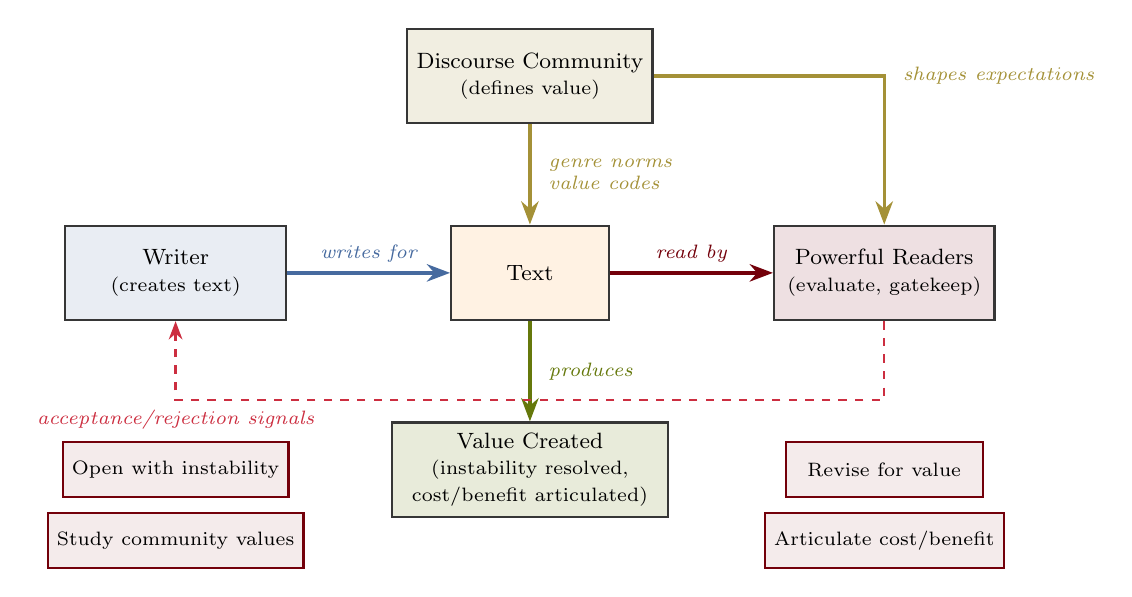
\begin{tikzpicture}[
    every node/.style={font=\footnotesize},
    mainbox/.style={rectangle, draw=black90, thick, minimum width=2.8cm,
        minimum height=1.2cm, align=center, font=\footnotesize},
    process/.style={rectangle, draw=garnet, thick, fill=garnet!8,
        minimum width=2.5cm, minimum height=0.7cm, align=center, font=\scriptsize},
]

% Writer
\node[mainbox, fill=atlantic!12] (writer) at (-4.5, 0) {Writer\\{\scriptsize (creates text)}};

% Discourse community
\node[mainbox, fill=honeycomb!15] (community) at (0, 2.5) {Discourse Community\\{\scriptsize (defines value)}};

% Readers
\node[mainbox, fill=garnet!12] (readers) at (4.5, 0) {Powerful Readers\\{\scriptsize (evaluate, gatekeep)}};

% Value
\node[mainbox, fill=horseshoe!15, minimum width=3.5cm] (value) at (0, -2.5)
    {Value Created\\{\scriptsize (instability resolved,}\\{\scriptsize cost/benefit articulated)}};

% Text in center
\node[mainbox, fill=sandstorm, minimum width=2cm] (text) at (0, 0) {Text};

% Arrows
\draw[-{Stealth}, very thick, atlantic] (writer) -- (text)
    node[midway, above, font=\scriptsize\itshape] {writes for};
\draw[-{Stealth}, very thick, garnet] (text) -- (readers)
    node[midway, above, font=\scriptsize\itshape] {read by};
\draw[-{Stealth}, very thick, honeycomb] (community) -- (text)
    node[midway, right=0.1cm, font=\scriptsize\itshape, align=left] {genre norms\\value codes};
\draw[-{Stealth}, very thick, honeycomb] (community.east) -| (readers.north)
    node[midway, right=0.1cm, font=\scriptsize\itshape] {shapes expectations};
\draw[-{Stealth}, very thick, horseshoe] (text) -- (value)
    node[midway, right=0.1cm, font=\scriptsize\itshape] {produces};

% Feedback loop from readers to writer
\draw[-{Stealth}, thick, rose, dashed] (readers.south) -- ++(0,-1) -| (writer.south)
    node[midway, below, font=\scriptsize\itshape] {acceptance/rejection signals};

% Key techniques annotations
\node[process] at (-4.5, -2.5) {Open with instability};
\node[process] at (-4.5, -3.4) {Study community values};
\node[process] at (4.5, -2.5) {Revise for value};
\node[process] at (4.5, -3.4) {Articulate cost/benefit};

\end{tikzpicture}
\end{document}
